\subsection{Razonamiento de Contexto}
\label{subsec:Prop_Razonamiento}


\subsubsection{MODIFICACIÓN}

CAMBIARÁ RADICALMENTE

Se propone el uso de SPARQL como en el artículo \cite{Meditskos2013, Meditskos2016}
Hay una nueva versión pero aún no está soportada.


Drools para filtrar las posibilidades y no sobrecargar la ontología, reglas ontológicas para actuar directamente sobre el dominio (actividades que se pueden seleccionar) \textbf{CITAS DE QUE ES NECESARIO DISMINUIR LA CARGA EN EL RAZONADOR} \cite{Ordonez2016}, \cite{Hille} - parece que el ontológico es mejor pero no hablan de si desempeño.

proceso 

reglas generales (Drools) --- - -- reglas dom (SWRL)

Esta capa se permite identificar las acciones más relevantes para el usuario a partir de dos componentes de gran importancia una ontología de alto nivel y una base de datos que contiene ontologías y reglas para cada dominio. El uso de ontologías de alto nivel permite disminuir de la carga de procesamiento del razonador y la independencia de la información que se está manejando (división de la información), trabajos como (PONER TRABAJO) usan dos o más ontologías para representar el conocimiento. En este trabajo se propone el uso de dos sistemas de reglas lógicas (i) las reglas de tipo 1 (RT1) \textbf{SWRL} (PONER REFERENCIA AL ESTANDAR) que actuarán sobre las clases y relaciones existentes en la ontología para definir el contexto del usuario, y (ii) las reglas de tipo 2 (RT2) \textbf{Drools (RT2)} con las que es posible modificar el comportamiento de los servicios dependiendo de los atributos encontrados en el contexto. Gracias a la división de las reglas se puede omitir el modelado de los servicios dentro de la ontología de contexto pues las reglas de tipo SWRL actuan solo sobre componentes de la ontología.

El proceso de selección de condiciones se conforma de seis etapas: 

\begin{enumerate}
    \item Filtrado de acciones no relevantes: a partir de la información resultante del razonamiento en la ontología se eliminan las reglas RT1 con lo que se disminuye la cantidad de opciones que deben ser verificadas.
    \item Revisión de las reglas del dominio: se comprueban las RT1 restantes y se obtienen los atributos de contexto identificados, estos atributos de contexto normalmente representan actividades de alto nivel. 
    \item Selección de reglas: a partir de los datos de contexto se evalúan RT2 obteniendo todos los posibles servicios de respuesta del sistema.
    \item Organización de reglas: dado que se pueden obtener uno o mas servicios, estos se organizan de acuerdo al valor de preferencia para el usuario \textbf{(ESPECIFICAR CUALES)}.
    \item Creación del servicio: se envía el servicio a la distribución del contexto en donde se aplicarán las acciones a las entidades de contexto del sistema.
    \item Actualización de reglas: después de que el usuario ha interactuado con el dispositivo se actualizan las reglas y los valores de preferencia de estas.
\end{enumerate}

Se espera que cada uno de los dominios en los que puede actuar la aplicación esté modelado en una ontología y tenga sus propias reglas.
A continuación por medio de



% http://www.miningminds.re.kr/lifelog/context/context-v2.5.owl

Algunas ontologías de contexto son presentadas por
\cite{Bikakis2007}Sirve porque presenta una lista de ontologías de contexto que posiblemente ya no se encuentren habilitadas, dice también los diferentes tipos de razonamiento que existen

% Tengo dos pares que combinan linked data, cada par es de los mismos autores en el mismo año


% http://linkdata.org/ - POSIBLE HERRAMIENTA



% El razonamiento es -----, las formas comunes de razonamiento son : \cite{Bikakis2007}


% La mayoría encontrada usa ontológico y reglas DL (poner todos los artículos que lo hacen), lo anterior obedece a la falicidad de creación de las reglas pero, trabajos como BLA BLA los dos que hablan de métodos aparte señalan el problema del manejo de la incertidumbre que es cuando no se encuentra nada que siga las reglas.



\cite{Garcia-Sola2014} García propone un sistema de razonamiento distribuido que busca mejorar el desempeño de los razonadores ontológicos tomando pequeños fragmentos de la ontología y combinando diferentes métodos de razonamiento como reglas y representación de acciones en arboles.Aunque la propuesta es clara las tecnologías no son específicadas e indica que el cálculo de tiempo para seleccionar los diferentes métodos de razonamiento no es muy certero.

\cite{Avenoglu2017} Presenta un sistema sensible al contexto SOMNIUM que modela las actividades diarias del usuario como un flujo y utiliza reglas del tipo Drools. La información de contexto se usa solo cuando es pertinente dentro del flujo, disminuyendo \textbf{el peso} del procesamiento y recomendando acciones a los usuarios en tiempo real y de acuerdo su rutina. El esquema de la propuesta principal se divide en un componente que ejecuta y administra las actividades del usuario, un componente que ejecuta las reglas y dos componentes que permiten especializar el sistema de acuerdo al dominio en el que se va a ejecutar.



\cite{Iaz2014} 
having hybrid methods with a first data-driven preprocessing stage appears to be the right direction
to benefit from both data- and knowledge-driven computing paradigms.


% \cite{Li2017} Exploran el concepto de los sistemas sensibles al contexto en los submarinos robóticos, específicamente presenta una arquitectura para el razonamiento en sistemas de contexto que utiliza el razonamiento basado en ontologías, en reglas y en redes bayesianas. En esta propuesta se usa una ontología general, una que contiene datos del dominio y otra que se concentra en las aplicaciones o servicios que se pueden desarrollar. Este trabajo es bastante completo en la definición de la estratégia de razonamiento pues por medio del uso de las redes bayesianas logra eliminar la incertidumbre en el sistema de contexto cuando no hay información suficiente. 




% % https://github.com/ubiquitous-computing-lab/Mining-Minds/tree/master/information-curation-layer

% % https://jena.apache.org/getting_started/index.html


% El trabajo de Gu en el año 2004 mostraba un esfuerzo interesante por resolver problemáticas de los sistemas sensibles al contexto como la consistencia y el tiempo de razonamiento de las ontologías. En su propuesta, se presenta una arquitectura de tres capas (aplicación, razonamiento y adquisición de datos) y la ontología de contexto de alto nivel SOCAM que representa las entidades más importantes en los sistemas de contexto. El razonamiento de esta propuesta se da por medio de Logic Reasoning e inference rules \cite{Gu2004}.


% \cite{Chang2017} Presenta un modelo de contexto que tiene en cuenta datos de sensores variados con múltiples entidades como usuario, vehículo y carretera. Realiza el modelado de contexto por medio de ontologías y el razonamiento lo hace de la misma forma, solo que divide este proceso en 2 1 que permite encontrar la situación y otro (que entiendo no es razonamiento sino el uso de actividades guardadas en bases de datos) toma la decisión en el sistema de esta forma evita sobrecargar el mismo, también presenta datos de los tiempos que se demora el sistema en dar respuesta. El problema de este artículo es que no usa contenido multimedia, tampoco lo necesita, aunque tener información de música, texto y otras cosas puede facilitar la toma de decisiones (por ejemplo el uso del móvil en el proceso de conducción), también puede ser muy útil ver los procesos de interacción como multimedia.


% \cite{Razzaq2017} Este trabajo presenta el un componente de contexto para el framework Mining Minds el cual combina el uso de razonamiento con ontologías y MAchine Learning para obtener el contexto, lo anterior porque usar solo el razonamiento es bastante pesado. (no queda tan claro cómo usa la ontología ni tampoco cómo es el proceso de ML ya que es bastante general). Explica el uso de tecnologías cómo SPARQL, adicionalmente presenta una ontología que divide el contexto de alto y bajo nivel (puede servir de guia para el desarrollo de otras ontologías)  
% \cite{Wei2013} presenta una arquitectura para sistemas sensibles al contexto que adapta automáticamente las actividades que se presentan al usuario. Esta arquitectura usa ontologías y para el razonamiento Description Logic y First order logic reasoning. Para la toma de decisiones usa un proceso de filtrado en donde se eliminan primero las tasklets ménos importantes para el contexto y luego dependiendo de lo que sucede en el entorno se evaluan las opciones más optimas. esta propuesta no tiene encuenta los formatos y realiza razonamiento solo con las reglas de las ontologías




% Adaptaciòn automàtica de las decisiones en un sistema sensible al contexto 3 capas - programación (estruct y leng prog), conocimiento (ontolo) y decisión

% Technol
% Composital adaptation
% Ontology
% Description logic/first-order logic reasoning.
% Pellet for description logic
% jess for first-order logic reasoning

% Ontologías
% * Contexto - modela entidades de contexto para compartir información de entornos dinámicos
% * Tareas - taras de un individuo y requerimientos para condiciones contextuales
% * Servicios - propiedades de los servicios sensibles al contexto y los requerimientos para las tareas.

% Decisiones
% Multistage normative decision model (algo como arbol) para elegir las diferentes alternativas para la selección de la tarea. Primero se filtra, luego
% Description logic/first-order logic

% Presenta buenas gráficas de performance


% \cite{Wang}Presenta la creación de una ontología de contexto a partir de la caracterización de entidades como localización, usuario, actividad y computador. Dentro de esta propuesta se presenta también un ejemplo dónde se puede evidenciar el uso de reglas de razonamiento para encontrar contexto a partir de datos de entrada. (leer bien)  

Dadas las problematicas encontradas en el uso de SWRL entre las cuales se encuentra
\textbf{\textit{(i)}} tiempos largos de ejecución del paquete de reglas.
\textbf{\textit{(ii)}} falta de una característica que permita generar instancias en la ontología de forma automática.
Es claro que estas desventajas pueden darse debido al proceso generado para la ejecución de reglas en dos fragmentos.

\subsection{Ontología de Reglas}
\label{subsec:Prop_Razonamiento_Rules_Ont}

\begin{figure}[!ht]
    \centering%
    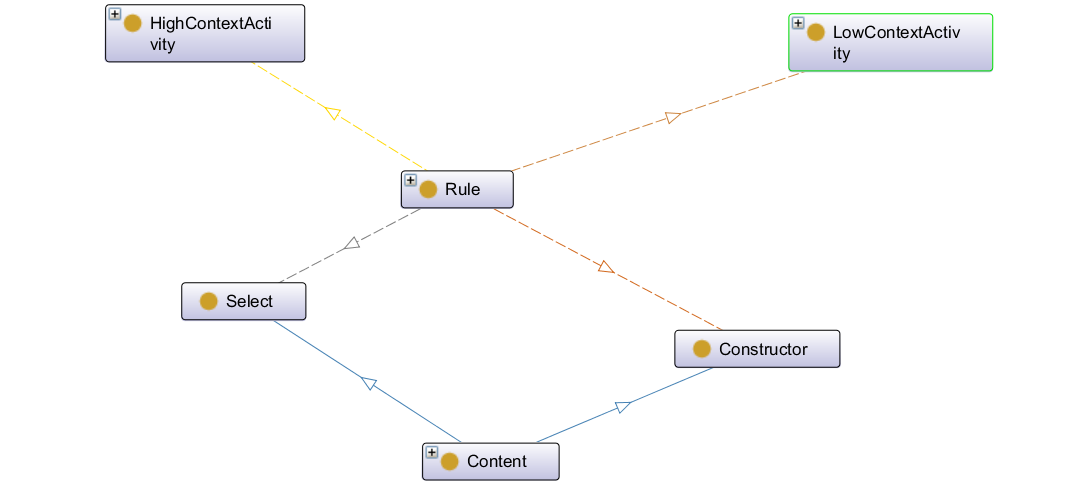
\includegraphics[width=0.3\textwidth]{Cap3/Images/Contexto_Razonamiento_Ont_Rules}%
    \caption{Ontología de Reglas.} \label{fig:Contexto_Razonamiento_Ont_Rules}
\end{figure}

Se crea una ontología, \ref{fig:Contexto_Razonamiento_Ont_Rules} que busca relacionar las actividades de contexto de alto y bajo nivel, presentadas en la ontología de la sección \ref{subsubsec:Prop_Mod_mContext}, con las reglas del dominio.

\subsection{Reglas SPARQL}
\label{subsec:Prop_Razonamiento_SPARQL}

Teniendo en cuenta el rendimiento ofrecido por las reglas SWRL se opta por una alternativa con SPARQL. En la figura \ref{fig:Flujo_reglas_sparql} se puede observar el flujo de aplicación de reglas el cual sigue los siguientes pasos:

\begin{itemize}
    \item 1) Se obtienen las actividades generadas en a un rango específico de tiempo, pueden ser las actividades de un día o las actividades de una hora determinada.
    \item 2) Se busca en el grafo de reglas aquellas instancias que tienen una relación con las actividades por medio de la propiedad isTrigger de la ontología de reglas \ref{subsec:Prop_Razonamiento_Rules_Ont}.
    \item 3) Se extraen los comandos construct y select que conformarán los queries SPARQL a ejecutar en el siguiente paso.
    \item 4) Se ejecutan las reglas y se generan las instancias y propiedades pertinentes.
\end{itemize}

Esta propuesta trata aspectos que no son mencionados por \cite{Meditskos2013} como:
\textbf{\textit{(i)}} manejo de un gran número de reglas en la bd de grafos - en el trabajo no es claro como se realiza la ejecución de cada una de las reglas en el sistema, si se ejecutan todas las posibles o se realiza algún tipo de filtrado.
\textbf{\textit{(ii)}} representación de las reglas en un grafo para la recuperación eficiente de acuerdo a diferentes elementos de la ontología del dominio.
\textbf{\textit{(iii)}} es posible agregar mas componentes a las reglas como lugar o acompañante.

\todo{TABLA DE COMPARACIÓN ENTRE EL USO DE REGLAS CON SWRL Y SPARQL}